\documentclass[12pt]{article}

\usepackage{geometry}   % To control page margins
\usepackage{fancyhdr}   % To customize the header and footer
\usepackage{enumitem}   % For better lists
\usepackage{setspace}   % For line spacing
\usepackage{parskip}    % For better paragraph spacing
\usepackage{graphicx} % inserting images


\geometry{a4paper, margin=1in}

\pagestyle{fancy}
\fancyhf{}
\fancyhead[L]{Data Warehouses} 
\fancyfoot[C]{\thepage}

\title{Introduction to Data Warehouses}
\author{0xSaad / Saad Almalki}
\date{\today}

\begin{document}

\maketitle

\textbf{Data warehouse :} is constructed by Integrating data from multiple heterogeneous sources that supports Analytical reporting and Decision making .

Data Warehousing involves :

\begin{itemize}
    \item Data Cleansing
    \item Data Integration
    \item Data Consolidations

    
\end{itemize}

\section{Business Intelligence}

Transformation \textbf{Data} to \textbf{Information}

Then

Derivation \textbf{Knowledge} from \textbf{Information}

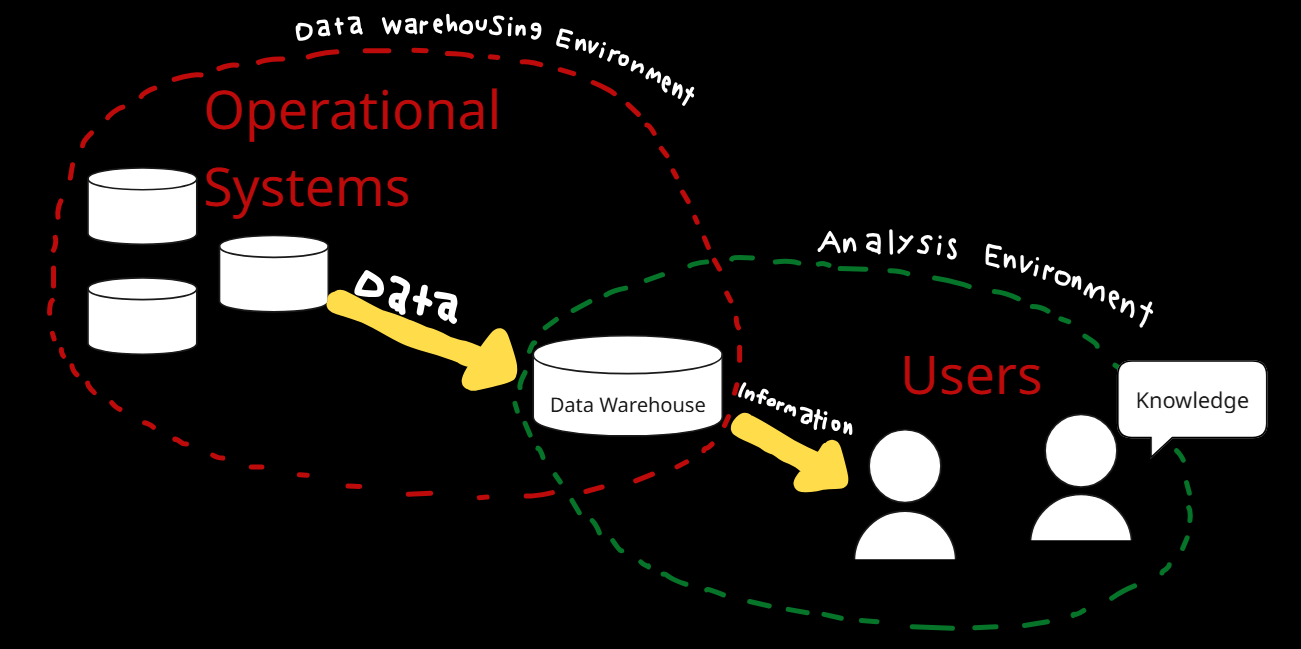
\includegraphics[width=0.5\textwidth]{images/datawarehouse.png} \\

\section{Query Driven Approach}

This is traditional approach to integrate heterogenous databases.

\subsection{Disadvantages :}

\begin{enumerate}


\item Need complex integration and filtering processes

\item Very inefficent

\item Very expensive for frequent queries

\item Very expensive for queries need to aggregations.

\end{enumerate}


\section{Update Driven Approach}
Alternative to traditional approach , Must of modern data warehouses systems used this approach more than query-driven approach.

\subsection{Advantages :}

\begin{enumerate}


\item Provides high performance

\item data is copied, processed, integrated, annotated, summarized 
and restructured in semantic data store

\item Query processing does not require an interface to process data at 
local sources

\end{enumerate}


\section{OLAP vs OLTP}

OLAP is \textbf{OnLine Analytical Processing} which refers to processing at warehouses

OLTP is \textbf{OnLine Transactions Processing} which refers to processing at operational systems 'databases' .

\subsection{OLTP}

\begin{enumerate}


\item Thousands of Users

\item Mostly updates

\item MBs or GBs of data

\item Raw Data

\item Many small transactions

\end{enumerate}

\subsection{OLAP}

\begin{enumerate}

\item Hundreds of Users

\item Mostly reads

\item Provides a History

\item GBs or TBs of data

\item Queries are long and complex

\end{enumerate}


\section{Useful resources}

The data warehousing institute: www.tdwi.org

Data warehousing on web :

\begin{itemize}


\item www.datawarehousing.org
\item www.datawarehousing.com

\end{itemize}


Online Magazines and Periodicals :

\begin{itemize}


\item www.intelligententerprise.com
\item www.dmgreview.com
\item www.cio.com

\end{itemize}


\begin{flushright}
Created by: Saad Almalki \\
\end{flushright}

\end{document}
